\documentclass[a4paper, 12pt]{article}
\usepackage{geometry}
\usepackage{setspace}
\usepackage{amsmath, amssymb}
\usepackage{amsthm}
\usepackage{thmtools}
\usepackage{hyperref}
\usepackage[portuguese, ruled, noend]{algorithm2e}
\usepackage{pgfplots}
\usepackage{caption}
\usepackage{subcaption}
\usepackage{graphicx}
\usepackage[utf8]{inputenc}
\usepackage[brazil]{babel}

\geometry{a4paper, margin=2.4cm}

\graphicspath{{./images/}}

\SetKwFor{Para}{para}{faça}{fim para}
\SetKwBlock{Inicio}{In\'{i}cio}{fim}

\declaretheorem[style=definition, name=Definição]{definicao}

\hyphenation{com-ple-xi-da-de}
\hyphenation{ca-mi-nho}
\hyphenation{des-pen-di-das}
\hyphenation{ge-ra-dos}

\title{Relatório Final de Projeto}
\author{Plácido Francisco de Assis Andrade\\ 
	\texttt{placido.andrade@ufca.edu.br} 
	\and 
	Ikaro Ruan Penha Costa \\
	\texttt{ikaroruan@outlook.com}
	}
\date{}

\begin{document}
\maketitle


\section*{Identificação de Projeto}
\textbf{Título} \\
Análise Quantitativa de PPC's \\

\noindent \textbf{Edital de Referência} \\
Edital Unificado 01/2017 \\

\section*{Área do Conhecimento Predominante}
Ciência da Computação

\onehalfspace
\section*{Resumo}

É certo que as Diretrizes Curriculares Nacionais regem os conteúdos que constituem os PPC's das Instituições de Ensino Superior do Brasil. Sendo assim, não 
é viável uma análise da pertinência de conteúdos de um curso de ensino superior, mas é possível proceder-se com um estudo do quão extenso ou profundo é a 
estrutura de um PPC. Logo, dois índices são propostos, os quais quantificam a complexidade e a possível retenção de alunos provenientes dos pré-requisitos da 
matriz curricular de um curso. Ainda, alguns parâmetros para construção dos índices são calculados e podem ser usados para a análise quantitativa do PPC, os quais 
foram indicados como sub-índices. Foi desenvolvido um aplicativo computacional de distribuição gratuita intitulado AnálisePPC como suporte para realização de 
simulações e comparação de matrizes curriculares semelhantes. Portanto, este projeto possibilita comparar tais índices com problemas acadêmicos enfrentados em diversos 
cursos, como evasão, abandono, repetência ou tracamento e simular possíveis situações visando diminuição da complexidade e retenção causada por pré-requisitos. \\

\textbf{Palavras-chave:} Estrutura curricular. Análise quantitativa. PPC. IES. AnálisePPC.

\section*{Introdução}

No processo de criação de um Projeto Político-pedagógico de Curso (PPC), a atenção prioritária é posta nos conteúdos a serem integralizados, sendo os maiores parâmetros 
observados as Diretrizes Curriculares Nacionais estabelecidas pelo Conselho Nacional de Educação (CNE) do Ministério da Educação. Esta é uma postura natural e 
não cabe, assim, observar a conveniência dos conteúdos propostos, mas torna-se interessante a análise quantitativa de fatores como a extensão do curso, a 
profundidade e a quantidade de cominhos de pré-requisitos da estrutura curricular, as cargas horárias complementares e de estágio obrigatório. \\

Para tal análise são propostos parâmetros, sub-índices, para a construção do dois índices em estudo neste trabalho: Índice de Retenção e Índice de Complexidade. 
Tomando-se um turno de um estudante com carga horária diária de oito horas, sendo quatro horas despendidas em aulas teóricas e práticas e outras quatro em 
estudo individual, pode-se compor o sub-índice dos Turnos Efetivos como a quantidade de turnos exigidos por semestre em um PPC. A ideia principal do 
sub-índice do Peso dos Pré-requisitos considera a extensão dos caminhos de pré-requisitos e se estes estão em semestres consecutivos, visto que quanto mais 
longo um caminho e mais concentrado em semestre consecutivos maior é o seu peso, visando a integralização do curso. Ainda, quantificando a recorrência de um 
pré-requisito e diferentes caminhos, pode-se formar os Pré-requisitos Acumulados. Ao se unir tais parâmetros, pode-se construir o Índice de Complexidade, 
o qual considera os três parâmetros anteriores, e o Índice de Retenção que contempla a disposição das disciplinas ao longo dos semestres. \\

Como ferramenta para o cálculo de tais índices foi desenvolvido um programa computacional intitulado AnálisePPC. O seu algoritmo interpreta o PPC como 
um Grafo Acíclico Direcionado (\textit{DAG}, sigla em inglês), em que cada vértice é tido como uma disciplina e cada aresta indica a necessidade de integralizar 
uma disciplina para se poder cursar a disciplina subsequente. Dessa forma, pode-se percorrer o grafo em busca dos caminhos de pré-requisitos possíveis e, então, 
calcular os índices propostos. \\

Portanto, o programa AnálisePPC pode servir como uma útil ferramenta para os conselhos de cursos e de criação de PPC's das Instituições de Ensino Superior 
do Brasil. Possibilitando simulações por diversas alterações na estrutura curricular de curso de ensino superior. O AnálisePPC embasa as mudanças em complexidade e 
retenção do curso, afetando diretamente o discente, em decorrência da criação ou modificação de PPC's. Sendo assim, este projeto pode servir para 
busca de melhorias quanto aos problemas de evasão, repetência, abandono ou trancamento.

\section*{Justificativa}

Os autores do trabalho não têm ciência quanto a análises semelhantes da estrutura curricular de um PPC ou quanto ao \textit{software} em trabalhos 
prévios. Logo, a sua execução justifica-se por possibilitar além da análise quantitativa como ferramenta para criação e modificação de PPC's, 
mas também pode-se atribuir uma linha de pesquisa relacionada à ensino-aprendizagem na educação superior brasileira.

\section*{Referencial Teórico}
Como mencionado anteriormente, os autores não tem conhecimento de um trabalho anterior com análise semelhante de um PPC. Assim, os índices a serem apresentados 
a seguir foram propostos e refinados pelos autores até a sua consolidação. \\ 

Por sua essencialidade na construção dos índices, os sub-índices Turnos Efetivos, Peso dos Pré-requitos e Pré-requisitos Acumulados terão sua formulação 
matemática apresentada. Em seguida, os Índices de Complexidade e Retenção serão definidos.

\subsection*{Turnos Efetivos ($\mathcal{T}_{ppc}$)}
Toma-se por aluno padrão aquele referente a interpretação de um estudante como um profissinal engajado em uma carga horária de 8 horas por dia, sendo 
4 horas despendidas em aulas teóricas e práticas e 4 horas de estudo individual. Considera-se, ainda, que o aluno padrão tem carga horária semestral de 
$T_0 = 320h$ de aulas teóricas e práticas distribuídas em 100 dias letivos. \\ 

Para a definição do Turno Efetivo serão utilizadas as gradezas apresentadas a seguir: \\

\begin{enumerate}
\item $n$: número de semestres propostos para integralização.
\item $M_{ppc}$: carga horária de integralização do PPC.
\item $M_{ac}$: carga horária de integralização das atividades complementares.
\item $M_{est}$: carga horária de estágio supervisionado.
\item $s_i$: semestre letivo $i$.
\item $M_i$: soma das cargas horárias das disciplinas alocadas no semestre $s_i$.
\end{enumerate}

\begin{definicao}
A quantidade de turno efetivo do semestre $s_i$ de um PPC com uma proposta de $n$ semestres  de integralização é \\

$$\tau_i = 2\frac{M_i}{T_0} + \frac{\frac{M_{ac}+M_{est}}{n}}{T_0}$$
\end{definicao}

\begin{definicao}
A quantidade de turnos efetivos do PPC com $n$ semestres letivos de integralização é \\
$$\mathcal{T}_{ppc} = \sum_{i = 1}^{n} \tau_i$$
\end{definicao}

\subsection*{Peso dos Pré-requisitos ($\mathcal{P}_{ppc}$)}

Inicialmente, deve-se conceituar um caminho de pré-requisitos. Dá-se à sequência $\alpha = \{ (m_i, s_i) \}_{i=1}^k$ a designação de um caminho de 
pré-requisitos sendo $m_i$ a carga horária e $s_i$ o semestre proposto da disciplina $d_i$. Atenta-se, pois, que a disciplina $(m_i, s_i)$ é um pré-requisito 
para $(m_{i+1}, s_{i+1})$. \\ 

O julgamento da dificuldade de uma disciplina é um processo subjetivo, não cabendo aqui a sua utilização. Logo, não é justo afirmar que uma disciplina de 
maior carga horária é de maior complexidade. Por outro lado, é possível assumir que uma disciplina alocada em um semestre mais avançado terá maior peso no 
tempo integralização previsto, haja vista que a perda de tal disciplina por algum motivo acarreta em menor tempo para recuperação do atraso causado.
Sendo assim, atribui-se o maior peso de um caminho $\alpha$ o valor do semestre $s_k$. \\

Ainda considerando o tempo necessário para recuperação do atraso causado pela perda de uma disciplina, considera-se que disciplinas consecutivas tenha o 
mesmo peso, pois a perda de uma delas resulta em uma reação em cadeia incrementando o valor dos seus semestres. Atribui-se, então, que todas as disciplinas 
consecutivas tem peso igual ao maior valor de semestre entre elas. \\

Isto significa que para duas disciplinas $(m_i, s_i)$ e $(m_j, s_j)$ presentes em um caminho $\alpha$, se $s_i - s_j = i - j$ então as duas disciplinas 
terão peso equivalentes de valor igual a $\max{\{ s_i, s_j \}}$. \\

Seja $\mathcal{S}_\alpha = {s_1, s_2, \ldots, s_k}$ o conjunto constituído pelos semestres do caminho $\alpha$. Define-se a relação de equivalência em 
$\mathcal{S}_\alpha$, 

$$ s_i \equiv s_j \qquad \text{se, e somente se, } \qquad s_i - s_j = i - j. $$

Para a definição do Peso dos Pré-requisitos, toma-se $Q_\alpha = \{ Q_{i_1}, Q_{i_2}, \ldots, Q_{i_p} \}$ de modo que $i_1 < i_2 < \cdots < i_p$ como 
o conjunto das classes de equivalências de $\mathcal{S}_\alpha$ e $s_{i_j} = \max Q_{i_j}$ para todo $j$ tal que $1 \leq j \leq p$. \\

Com efeito, sendo $\#Q_{i_j}$ a cardinalidade do conjunto $Q_{i_j}$ e $\log{x}$ o logaritmo na base 10, verifica-se

\begin{definicao}
Seja $\alpha$ um caminho de pré-requisitos, o Peso dos Pré-requisitos das disciplinas do caminho $\alpha$ é
$$ \mathcal{P}_\alpha = \sum_{j=1}^p (\#Q_{i_j}\log{s_{i_j}}) $$
\end{definicao}


\subsection*{Pré-requisitos Acumulados $(\mathcal{R}_{ppc})$}
Um mesmo pré-requisito pode aparecer em diversos caminhos de pré-requisitos diferentes, em que isso é causado pelas bifurcações causadas 
por disciplinas que são pré-requisitos para mais de uma disciplina posterior. Isto indica que as disciplinas antes das bifurcações são essenciais 
para a integralização do curso no tempo proposto no PPC. \\

Procurando-se contabilizar a importância de tais disciplinas presentes em diversos caminhos, conta-se a quantidade de pré-requisitos em cada 
caminho do PPC. Sendo $\alpha$ um caminho de pré-requisitos, $||\alpha||$ é número de disciplinas do caminho. Seja $\Gamma$ o conjunto de todos 
os caminhos do PPC, define-se:

\begin{definicao}
O número de pré-requisitos presentes no caminho $\alpha$, denotado por $\mathcal{R}_\alpha$, é

$$ \mathcal{R}_\alpha = ||\alpha|| - 1 $$
\end{definicao}

\begin{definicao}
O número de pré-requisitos acumulados presentes no PPC é
$$ \mathcal{R}_{ppc} = \sum_{\alpha \in \Gamma} \mathcal{R}_\alpha $$
\end{definicao}

\section*{Índice de Complexidade ($\Delta_{ppc}$)}
Pode-se considerar que a quantidade de horas requeridas de estudo por um curso de ensino superior, a composição das disciplinas e seus pré-requisitos, assim 
como a influência que exercem os pré-requisitos na integralização proposto na grade curricular são fatores que contribuem para maior ou menor complexidade 
de um PPC. Sendo assim, define-se: 

\begin{definicao}
O índice de complexidade de um PPC, denotado por $\Delta_{ppc}$, é a soma de turnos efetivos, peso dos pré-requisitos e pré-requisitos acumulados, ou seja,

$$\Delta_{ppc} = \mathcal{T}_{ppc} + \mathcal{P}_{ppc} + \mathcal{R}_{ppc}$$
\end{definicao}

\section*{Índice de Retenção ($\gamma_{ppc}$)}

Cabe à administração do curso a programação semestral das disciplinas do curso, assim como a disposição de cada disciplina na grade de horário semanal. O 
Índice de Complexidade não considera questões como reprovação, oferta de disciplina e tempo de conclusão. Duas hipóteses sobre a administração do curso 
são feitas visando modelar tais questões.

\begin{enumerate}
\item As disciplinas são ofertadas anualmente com semestralidades indicadas no PPC.
\item O aluno terá sucesso ao cursar pela segunda vez uma disciplina. 
\end{enumerate}

Suponha $d$ uma disciplina a qual um aluno, por algum motivo, não realizou sua matrícula ou foi reprovado. Sendo as disciplinas do curso de oferta anual, 
$d$ será deslocada dois semestres a frente. Ademais, considerando os caminhos de pré-requisitos $\beta$ que contém $d$, todas as disciplinas a frente de 
$d$ em $\beta$ também serão deslocadas em dois semestres. Logo, o caminho de pré-requisitos retificado seria na forma:

$$ \beta_{ret}: (m_1, s_1 + 2) \rightarrow (m_2, s_2 + 2) \rightarrow \cdots \rightarrow (m_k, m_k +2) $$

Seja $\Gamma(d)$ o conjunto constituído por os todos os sub-caminhos com início em $d$. Como definido anteriormente, $\mathcal{S}_\beta$ e 
$\mathcal{S}_{\beta_{ret}}$ são os conjuntos dos semestres, assim como $Q_\beta$ e $Q_{\beta_{ret}}$ as respectivas classes de 
equivalência. Observa-se que $Q_{\beta_{ret}}$ é obtido somando-se 2 a cada elemento de $Q_\beta$.

\begin{definicao}
O Índice de Retenção de uma disciplina $d$ em relação a um sub-caminho $\beta \in \Gamma(d)$ é

$$ \gamma_{\beta} = \sum_{j = 1}^{p}(\#Q_{k_j} \log(s_{k_j}+2)) $$
\end{definicao}

\begin{definicao}
O Índice de Retenção de uma disciplina é

$$ \gamma_d = \sum_{\beta \in \Gamma(d)} \gamma_\beta $$
\end{definicao}

\begin{definicao}
O Índice de Retenção de um PPC é

$$ \gamma_{ppc} = \sum_{d} \gamma_d $$
onde o somatório percorre todas as disciplinas do PPC.
\end{definicao}

\section*{Objetivos}

O objetivo geral consiste do desenvolvimento de um software para a análise quantitativa de PPC's. Especificamente, pode-se ressaltar: 

\begin{enumerate}
\item Iniciar um estudante na construção de um aplicativo. (T)
\item Criar um aplicativo que seja útil aos gestores que lidam com o aspecto ensino-aprendizagem na UFCA. (T)
\item Fazer comparações entre PPC's dos cursos da UFCA com de outras instituições de ensino superior. (T)
\item Elaborar linhas de estudo sobre ensino-aprendizagem utilizando possíveis refinamentos da análise estabelecida inicialmente. (P)
\end{enumerate}

\section*{Metodologia}

\subsection*{Algoritmo}

Para armazenar o PPC e auxiliar o cálculo dos índices, foi utilizada uma estrutura de dados na forma de um Grafo. Em concordância com \cite{book_cormen} e \cite{book_sedgewick}, seja $G = (V, E)$ um grafo, consistindo de um conjunto finito de vértices $V$ e um conjunto finito de arestas $E$. Quando $E$ é 
composto por pares ordenados $(u, v)$ sendo $u, v \in V$ o grafo é chamado de \textit{direcionado}, logo $(u, v) \neq (v, u)$. \\

Define-se por caminho em um grafo $G$ como uma sequência de vértices $\alpha = \{ v_1, v_2, \dots, v_k \}$ tal que $(v_i, v_{i+1}) \in E$ para $i = 1, 2, \dots, k$.
Essa definição assemelha-se a de um caminho de pré-requisitos, sendo $d_i$ a disciplina de um PPC vista como um vértice do grafo $G$. Com efeito, sejam $d_1$ e 
$d_2$ disciplinas de um PPC, o par ordernado $(d_1, d_2)$ é uma aresta de $E$ com $d_1$, $d_2 \in V$, significando que a disciplina $d_1$ é um pré-requisito 
para $d_2$. \\

Ainda, os caminhos de um PPC são acíclicos, visto que disciplinas de semestres mais avançados não serão pré-requisitos para disciplinas de semestres 
anteriores. Ou seja, para qualquer caminho $\alpha$ de $G$ com $k$ vértices, este terá $k-1$ arestas, haja vista que sendo $d_i=(m_i, s_i)$ é pré-requisito para 
$d_j=(m_j, s_j)$, então $s_i > s_j$. Logo, o PPC toma a forma de Grafo Acíclico Direcionado (\textit{DAG}, do inglês Directed Acyclic Graph). \\

A forma computacional utilizada para armazenamento do grafo é a de lista de adjacências. Um arranjo principal tem como elementos informações que apontam para uma 
lista encadeada, a qual cada nó compõe um vértice e vértices adjacentes compõem as arestas do grafo. A Figura \ref{img:adjacencies_list} apresenta um 
esquema da lista de adjacências. \\

\begin{figure}[h]
\centering
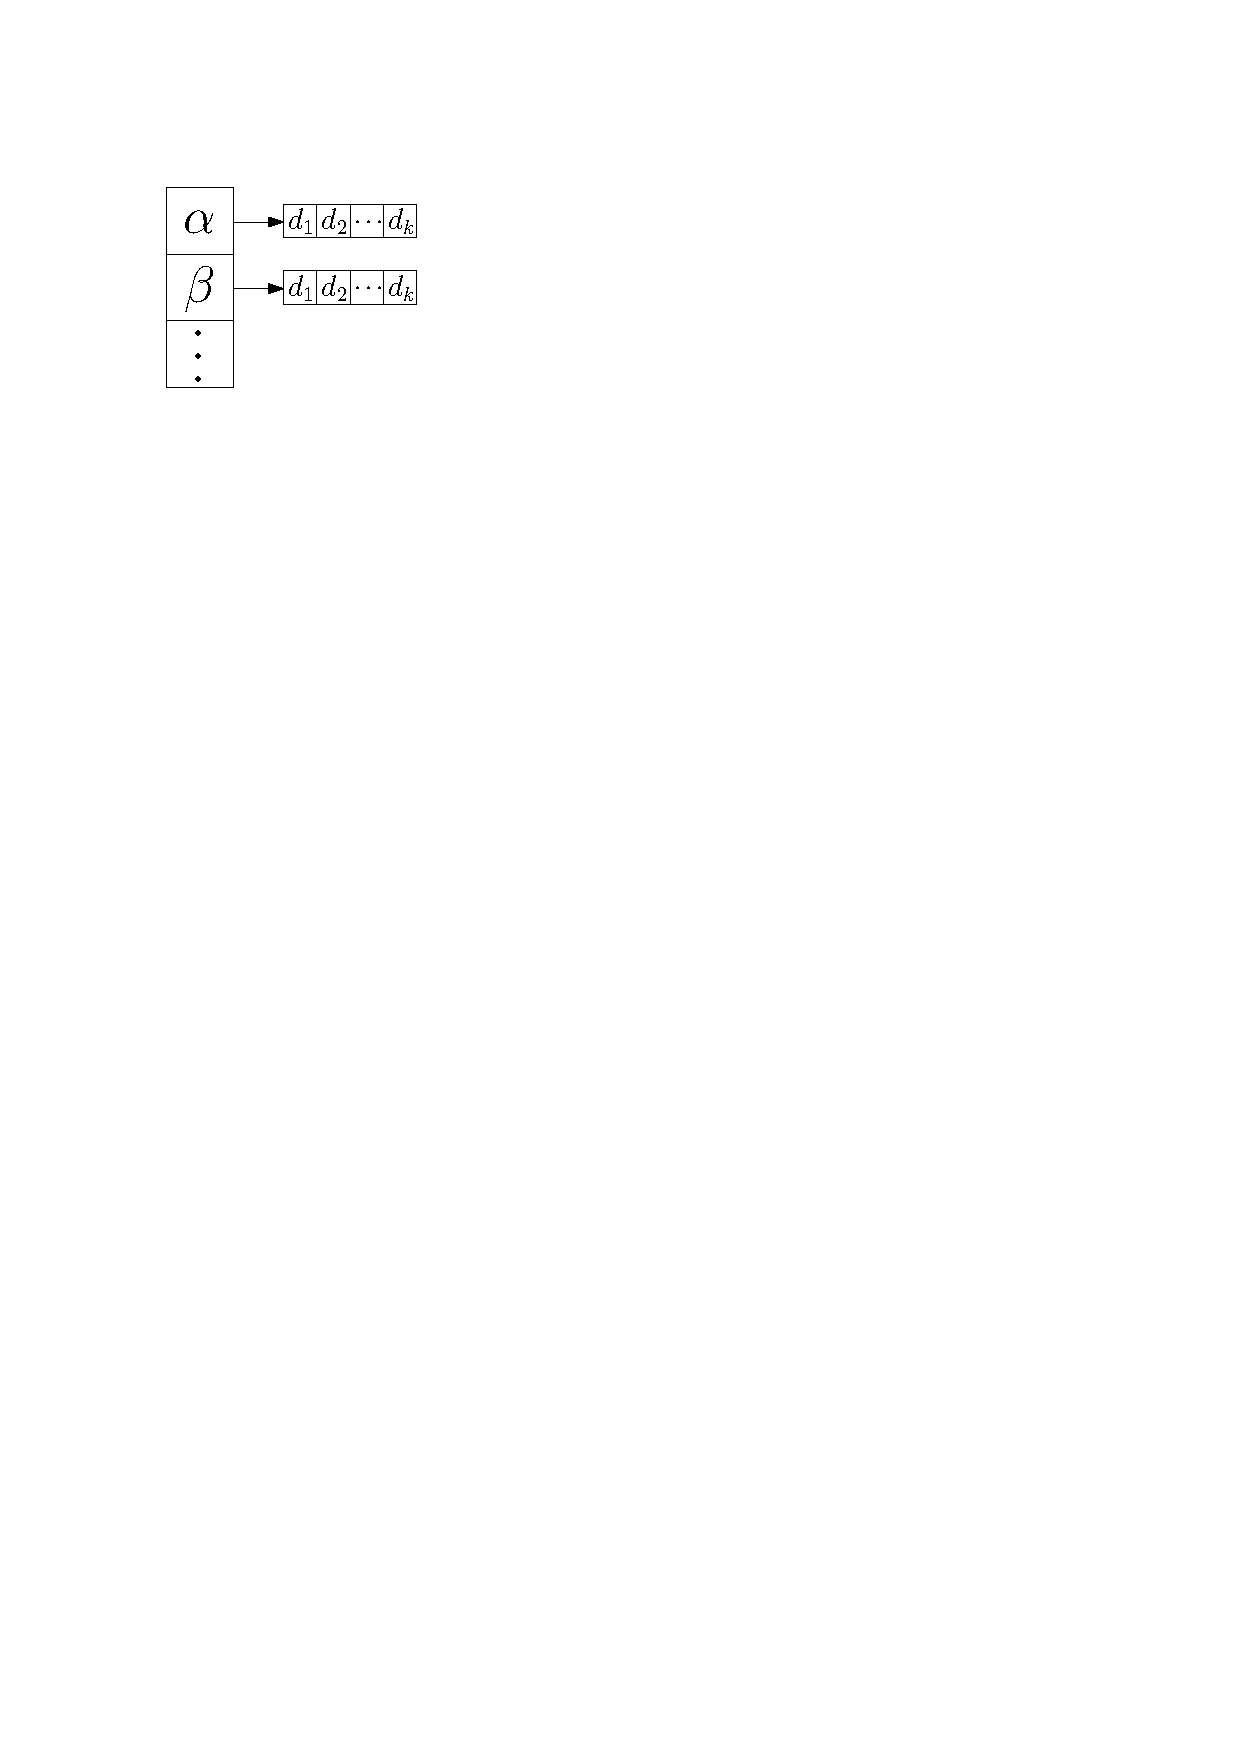
\includegraphics[scale=0.8]{adjcencies_list.pdf}
\caption{Esquema representativo de uma lista de adjacências.}
\label{img:adjacencies_list}
\end{figure}

Definindo um vértice raiz $d_R$ como sendo aquele que não possui pré-requisitos, ou seja, $d_R = (m_0, s_0)$ quando pertencente a um caminho $\alpha \in \Gamma$. Ainda, 
defini-se como vértice extremidade $d_E$ quando este não for pré-requisito para nenhuma outra disciplina do PPC, ou seja, $d_E = (m_k, s_k)$ para qualquer caminho 
$\alpha \in \Gamma$ de tamanho $k$, e uma bifurcação como um vértice que é pré-requisito para mais de uma disciplina. \\

Para a busca de todos caminhos possíveis em um grafo $G = (E, V)$, inicia-se com um vértice raiz e caminha-se em direção a outros vértices respeitando a relação de 
pré-requisitos entre as disciplinas até que um vértice extremidade seja atingido, então, se houve uma bifurcação $d_B$ no caminho formado, retorna-se a $d_B$ e 
procede-se da mesma maneira até atingir outro vértice extremidade, caso não haja 
birfurcação, o caminho já foi formado. Deve-se repetir o processo até que todos 
os vértices raiz tenham seus caminhos encontrados. O algoritmo é formalizado como a seguir. \\

\begin{algorithm}[H]
\small
\SetAlgoNoLine
\Entrada{Grafo $G=(E,V)$ com $V$ conjunto de vértices e $E$ conjunto de arestas.}
\Saida{Conjunto $\Gamma$ com os caminhos de $G$.}
\Inicio{
	Pilha $p$ com vértices raiz de $V$ \\
	\Enqto{$p$ não é vazia}{
		$d$ = frente de $p$ \\
		remova a frente de $p$ \\
		percorra as adjacências a partir de $p$ até uma extremidade \\
		adicione todos os vértices encontrado ao caminho $\alpha$ \\
		adicione $\alpha$ em $\Gamma$\\
		\Se{$\alpha$ possui bifurcação ainda não visitada}{
			adicione a bifurcação à pilha $p$
		}
	}
}
\Retorna{$\Gamma$}
\caption{DFS para caminhos de pré-requisitos.}
\end{algorithm}

Sob posse de todos os caminhos formados pelo PPC, pode-se calcular todos parâmetros necessários ao cálculo dos sub-índices, como as classes de equivalências do Peso 
dos Pré-requisitos. Logo, pode-se ter o resultado dos índices para o PPC. \\

Além disso, foram calculados os valores dos índices para cada semestre proposto para integralização com o intuito da construção de gráfico. Para tal, toma-se um 
semestre $s_i > 0$ e calcula-se os valores do Índice de Retenção e do Índice de Complexidade não levando em conta os semestres $s_j < s_i$, considerando que os 
semestres anteriores já foram integralizados.

\subsection*{Desenvolvimento}

Para o desenvolvimento do \textit{software} foi utilizada a linguagem Python 3 e a biblioteca nativa para salva e gerenciar o PPC em XML. Foi desenvolvida uma 
GUI (\textit{Guided User Interface}) através do PyQt 4 e Matplotlib para apresentação dos gráficos. \\ 

O aplicativo AnálisePPC foi desenvolvido em plataforma Linux. Executáveis foram gerados a partir do PyInstaller 3.3 tanto para Windows como para Fedora e estão publicados em 
\url{analiseppc.github.io}. A janela principal é apresentada na Figura \ref{img:main-window}.

\begin{figure}[htb]
\centering
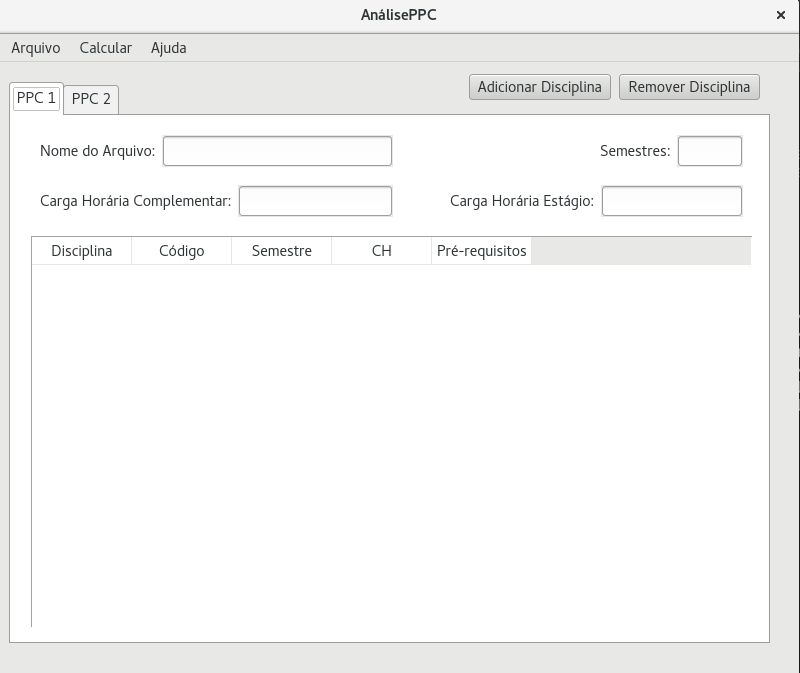
\includegraphics[scale=0.45]{main-window}
\caption{Janela principal do aplicativo AnálisePPC.}
\label{img:main-window}
\end{figure}

Para adicionar disciplinas, os dados necessários são requisitados a partir da janela como mostrada na Figura \ref{img:course-window}. Vale ressaltar que as 
disciplinas são organizadas por seus códigos. Logo, para inserir os pré-requisitos, deve-se inserir os códigos das disciplinas separadas por espaço simples. \\

\begin{figure}[h]
\centering
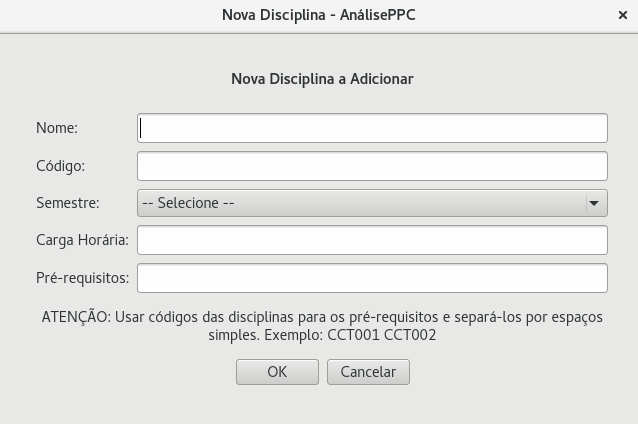
\includegraphics[scale=0.5]{course-window}
\caption{Janela para inserção dos dados da disciplina.}
\label{img:course-window}
\end{figure}

Como visto na Figura \ref{img:main-window}, é possível inserir e calcular dois PPC's simultâneos. Portanto, essa funcionalidade possibilita comparar diferentes 
documentos ou realizar simulações a partir de alterações de um mesmo PPC. Frizando que a opção de comparação mostra os resultados para os dois arquivos em 
uma mesm janela. \\

\section*{Resultados e Discussão}

Inicialmente, optou-se por realizar simulações com os PPC's dos cursos da UFCA. Para tal, foram aproveitados aqueles que sofreram reformulações nos últimos anos. 
Logo, serão analisados os PPC's dos cursos de Engenharia Civil e Administração 
Pública e Gestão Social. \\

Para o curso de Engenharia Civil foram analisados os ducumentos de 2008 e 2018. Os dois possuem mesmo número de semestres proposto para integralização. Contudo, 
o mais recente possui mair carga horária de integralização e menor valor requerido para carga horária complementar. A Figura \ref{img:civil-window} demonstra a visualização de resultados no AnálisePPC. Em seguida, temos expressos os valores 
para os índices de cada PPC. \\

\begin{figure}[htb!]
\centering
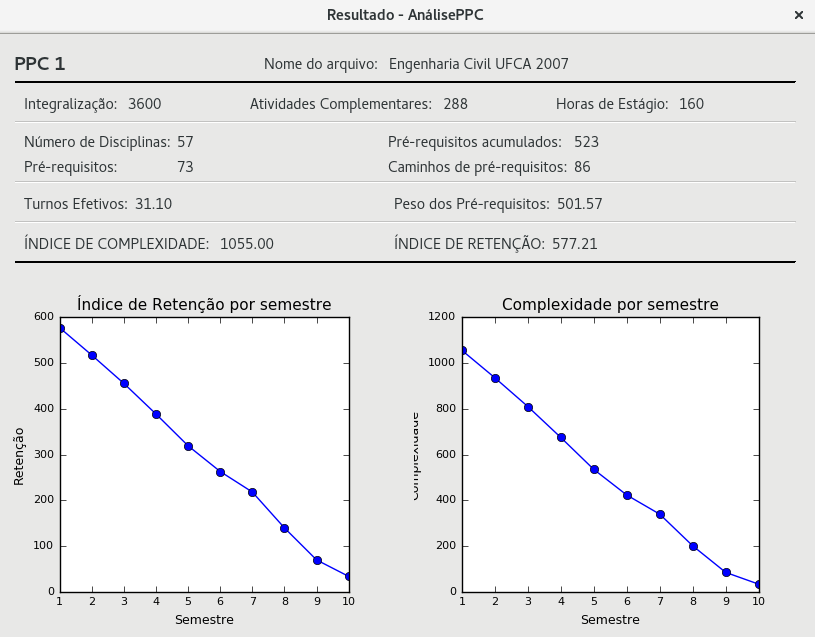
\includegraphics[scale=0.45]{civil-window}
\caption{Visualização dos resultados com o software AnálisePPC.}
\label{img:civil-window}
\end{figure}

Contudo, apesar do aumento na integralização e no número de disciplinas, o PPC de 2018 \cite{eng-civil2018} possui menores valores para o Índice de Retenção e o Índice de 
Complexidade. Isto se deve ao fato do grade curricular mais recente ter menor número de bifurcações, incorrendo em menor número de caminhos. Pode-se, ainda, 
ressaltar que o PPC de 2008 \cite{eng-civil2008} possui uma quantidade considerável de disciplinas que são pré-requisitos para mais de duas disciplinas. Tal ramificação toma 
forma tanto na complexidade quanto na retenção da estrutura curricular do curso. 

\vfill

\begin{center}
\begin{table}
\centering
\begin{tabular}{|l|c|c|}
\hline
\multicolumn{3}{|c|}{Engenharia Civil} \\ 
\hline\hline
	& PPC 2008 & PPC 2018 \\
\hline
Turnos Efetivos ($\mathcal{T}_{ppc}$) & 31,10 & 32,55 \\
\hline
Peso dos Pré-requisitos ($\mathcal{P}_{ppc}$) & 501,57 & 234,93 \\
\hline
Pré-requisitos Acumulados ($\mathcal{R}_{ppc}$) & 523 & 256 \\
\hline
Índice de Complexidade ($\Delta_{ppc}$) & 1055,00 & 522,00 \\
\hline
Índice de Retenção ($\gamma_{ppc}$) & 577,21 & 279,45 \\ 
\hline
\end{tabular}
\caption{Resultados obtidos dos sub-índices e índices para o curso de Engenharia Civil}
\end{table}
\end{center}

\begin{figure}[htb!]
	\centering
	\begin{minipage}[hb]{0.45\textwidth}
	\begin{tikzpicture}[scale=0.8]
		\begin{axis}[
			xlabel={Semestre},
			ylabel={Índice de Retenção},
			xtick={1, 2, 3, 4, 5, 6, 7, 8, 9, 10},
			legend pos = north east,
		]
		\addplot[color=blue, mark=square,]
			coordinates{(1, 577.2149)(2, 517.3670)(3, 455.4280)(4, 388.4659)(5, 319.0128)
				    (6, 262.7727)(7, 217.8957)(8, 139.4786)(9, 69.4666)(10, 33.4546)};
		
		\addplot[color=red, mark=triangle,]
			coordinates{(1, 279.4523)(2, 244.0756)(3, 209.1970)(4, 175.3465)(5, 143.8290)
				    (6, 110.3645)(7, 80.5395)(8, 54.4001)(9, 22.9862)(10, 1.0792)};
		\legend{PPC 2008, PPC 2018}
		\end{axis}
	\end{tikzpicture}
	\end{minipage}
	\hfill
	\begin{minipage}[hb]{0.45\textwidth}
	\begin{tikzpicture}[scale=0.8]
		\begin{axis}[
			xlabel={Semestre},
			ylabel={Índice de Complexidade},
			xtick={1, 2, 3, 4, 5, 6, 7, 8, 9, 10},
			legend pos = north east,
		]
		\addplot[color=blue, mark=square,]
			coordinates{(1, 1055.6718)(2, 935.5068)(3, 809.7551)(4, 674.3770)(5, 534.6973)
				    (6, 422.3564)(7, 338.9731)(8, 200.4778)(9, 84.3564)(10, 32.94)};
		
		\addplot[color=red, mark=triangle,]
			coordinates{(1, 523.4818)(2, 450.9207)(3, 378.1719)(4, 306.3242)(5, 243.2775)
				    (6, 174.9892)(7, 119.4161)(8, 69.2772)(9, 27.2749)(10, 2.695)};
		\legend{PPC 2008, PPC 2018}
		\end{axis}
	\end{tikzpicture}
	\end{minipage}
\caption{Resultado comparativo dos índices por semestre para o curso de Engenharia Civil.}
\end{figure}

Quanto ao PPC do curso de Administração Pública e Gestão Social, foram analisados os documentos de 2010 e de 2016. O primeiro apresenta 8 semestres como 
proposta para integralização do curso, quanto o segundo 9 semestres. Há uma siginificativa mudança nas quantidades de pré-requisitos, sendo o PPC de 2016 o de 
menor número. Ainda, houve redução na carga horária requeria para 
estágio e para atividades complementares. \\

O número de disciplinas aumentou em uma disciplina e, apesar da diminuição em horas de estágio e atividades complementares, as cargas horárias das disciplinas aumentaram 
de modo a ser verificado na diferença de turnos efetivos para o documento de 2016, verificado na Tabela \ref{tab:adm-publica}. \\

Os pré-requisitos foram substancialmente reduzidos de 2010 \cite{adm-publica2010} para 2016 \cite{adm-publica2016}, como verificado no sub-índice de pré-requisitos acumulados na Tabela \ref{tab:adm-publica}. 
Vale ressaltar também o aumento no índices de Complexidade e Retenção, como anteriormente, causados pelas bifurcações. O PPC de 2010 possui sete bifurcações, 
sendo uma delas uma disciplina como pré-requisito para mais de duas outras, 
enquanto o PPC de 2016 consta apenas uma bifurcação simples. \\

A Figura \ref{img:porsemestre-adm-publica} apresenta uma interseção nos gráficos para ambos os índices entre o quarto e quinto semestre. Isto representa que 
a boa parte dos pré-requisitos do PPC 2016 estão distribuídos em semestres superiores a quatro, visto que a menor inclinação do gráfico indica menor variação 
dos pré-requisitos ao longo dos semestres iniciais. \\


\begin{center}
\begin{table}[h]
\centering
\begin{tabular}{|l|c|c|}
\hline
\multicolumn{3}{|c|}{Administração Pública e Gestão Social} \\ 
\hline\hline
	& PPC 2010 & PPC 2016 \\
\hline
Turnos Efetivos ($\mathcal{T}_{ppc}$) & 23,90 & 27,17 \\
\hline
Peso dos Pré-requisitos ($\mathcal{P}_{ppc}$) & 41,57 & 30,46 \\
\hline
Pré-requisitos Acumulados ($\mathcal{R}_{ppc}$) & 47 & 20 \\
\hline
Índice de Complexidade ($\Delta_{ppc}$) & 111,00 & 77,00 \\
\hline
Índice de Retenção ($\gamma_{ppc}$) & 56,10 & 39,91 \\ 
\hline
\end{tabular}
\caption{Resultados obtidos dos sub-índices e índices para o curso de Administração Pública e Gestão Social.}
\label{tab:adm-publica}
\end{table}
\end{center}


\begin{figure}[h]
	\centering
	\begin{minipage}[hb]{0.45\textwidth}
	\begin{tikzpicture}[scale=0.8]
		\begin{axis}[
			xlabel={Semestre},
			ylabel={Índice de Retenção},
			xtick={1, 2, 3, 4, 5, 6, 7, 8, 9},
			legend pos = north east,
		]
		\addplot[color=blue, mark=square,]
			coordinates{(1, 59.0978)(2, 49.4466)(3, 42.1019)(4, 33.1722)(5, 25.3237)
				    (6, 20.1951)(7, 13.7712)(8, 9.0)};
		
		\addplot[color=red, mark=triangle,]
			coordinates{(1, 39.9140)(2, 36.3242)(3, 33.3139)(4, 29.0409)(5, 25.1502)
				    (6, 19.8476)(7, 16.2353)(8, 12.3311)(9, 7.2897)};
		\legend{PPC 2010, PPC 2016}
		\end{axis}
	\end{tikzpicture}
	\end{minipage}
	\hfill
	\begin{minipage}[hb]{0.45\textwidth}
	\begin{tikzpicture}[scale=0.8]
		\begin{axis}[
			xlabel={Semestre},
			ylabel={Índice de Complexidade},
			xtick={1, 2, 3, 4, 5, 6, 7, 8, 9},
			legend pos = north east,
		]
		\addplot[color=blue, mark=square,]
			coordinates{(1, 112.4706)(2, 95.2509)(3, 78.5718)(4, 56.8873)(5, 40.2573)
				    (6, 30.4718)(7, 18.1783)(8, 11.6403)};
		
		\addplot[color=red, mark=triangle,]
			coordinates{(1, 77.6392)(2, 68.9288)(3, 61.6153)(4, 52.2193)(5, 46.1007)
				    (6, 33.8818)(7, 26.0608)(8, 18.8630)(9, 10.5880)};
		\legend{PPC 2010, PPC 2016}
		\end{axis}
	\end{tikzpicture}
	\end{minipage}
\caption{Resultado comparativo dos índices por semestre para o curso de Engenharia Civil.}
\label{img:porsemestre-adm-publica}
\end{figure}

\vfill

\section*{Conclusão}

Mesmo não sendo objeto de estudo aqui a avaliação qualitativa de PPC's, os resultados obtidos demonstram que os índices quantitativos desenvolvidos são de 
significativa valia para gestores de cursos. Além disso, o aplicativo AnálisePPC torna mais prática a atividade de simular mudanças em estruturas curriculares 
e poder ter noção como tais mudanças podem afetar problemas acadêmicos como trancamento, desistência ou abandono de cursos. \\

Por conseguinte, AnálisePPC é uma ferramenta útil para gestores de cursos. Sendo assim, os autores almejam aplicar melhorias ao aplicativo com visualizações 
das estruturas curriculares do PPC, como também expandir a ideia a uma plataforma online em que diversas universidades possam compartilhar seus PPC's e 
ter disponível um banco de dados para possíveis comparações entre estruturas curriculares semelhantes.


\bibliographystyle{unsrt}
\bibliography{references}

\end{document}
